\section{Experimentación y resultados}
\label{sec:experimentacion}

Esta sección describe el equipo y el tamaño del problema, reporta la simulación del proceso de siembra en una hectárea, valida los dos métodos aproximados contra los exactos y presenta los resultados de los 30 polígonos. Todos los resultados se reproducen con \texttt{refor} y los scripts del repositorio del proyecto (\cref{sec:implementacion}), con la semilla 42.

\subsection{Características del equipo y del software}
\label{subsec:equipo}

Todos los experimentos se corrieron en el equipo de la \cref{tab:equipo}. Los programas se compilaron en modo de optimización (\texttt{Release}) y usan todos los núcleos disponibles; los resultados no dependen del número de hilos (\cref{subsec:impl-reproducibilidad}).

\begin{table}[t]
\centering
\caption{Equipo y software utilizados.}
\label{tab:equipo}
\small
\begin{tabularx}{\columnwidth}{@{}>{\RaggedRight\arraybackslash}p{2.5cm}>{\RaggedRight\arraybackslash}X@{}}
\toprule
Característica & Valor \\
\midrule
Modelo & MacBook Pro (Mac16,1) \\
Sistema operativo & macOS 26.5.2 \\
Disco duro & 494~GB, de estado sólido \\
Memoria RAM & 16~GB \\
Procesador & Apple M4 (ARM64) \\
Núcleos & 10 (4 de rendimiento y 6 de eficiencia) \\
\midrule
Lenguaje y compilador & C++20, Apple clang 17.0.0 \\
Construcción & CMake 4.3.0 \\
Solver entero & HiGHS 1.14.0 \\
Bibliotecas & CLI11 2.4.2, Catch2 3.7.1; Dear ImGui 1.92.8, ImPlot 1.0 y GLFW 3.4 (interfaz) \\
Análisis & Python 3.14.8 \\
Reporte & TeX Live 2025, pdf\TeX{} 1.40.27, Biber 2.20 \\
\bottomrule
\end{tabularx}
\end{table}

\subsection{Tamaño del problema}
\label{subsec:tamano}

La \cref{tab:tamano} resume el tamaño de la instancia. Hay 10 especies y una meta de 658 plantas por hectárea, que en los 30 polígonos suma 120{,}419 plantas; la composición del plan por especie está en la \cref{tab:compra-parametros} y la que resulta de la compra, en la \cref{tab:siembra}. En el nivel de compra, cada polígono tiene 20 variables enteras (una meta y una compra por especie); al resolverlo como mochila de elección múltiple hay una variable binaria por cada meta posible de cada especie, 24{,}094 en total, y las curvas que alimentan la mochila se estiman con 10{,}000 escenarios para cada uno de los 300 pares de polígono y especie. En el nivel espacial, el memético decide la especie de 52 posiciones por mosaico, y el modelo entero de cada mosaico tiene 520 variables binarias, 15{,}600 continuas y 3{,}182 restricciones.

\begin{table}[t]
\centering
\caption{Tamaño del problema. Los parámetros del modelo son datos o supuestos; los de los algoritmos controlan su ejecución.}
\label{tab:tamano}
\small
\begin{tabularx}{\columnwidth}{@{}>{\RaggedRight\arraybackslash}X r@{}}
\toprule
Elemento & Cantidad \\
\midrule
Especies & 10 \\
Polígonos (superficie total) & 30 (183.01~ha) \\
Plantas por hectárea (meta) & 658 \\
Meta total en los 30 polígonos & 120{,}419 \\
Plantas existentes registradas & 23{,}569 \\
\midrule
\multicolumn{2}{@{}l}{\textit{Variables}} \\
Compra: metas y compras por polígono & 20 \\
Compra: total en los 30 polígonos & 600 \\
Mochila: binarias en los 30 polígonos & 24{,}094 \\
Escenarios Monte Carlo por curva & 10{,}000 \\
Espacial: posiciones por mosaico & 52 \\
Modelo entero: binarias / continuas & 520 / 15{,}600 \\
Modelo entero: restricciones & 3{,}182 \\
\midrule
\multicolumn{2}{@{}l}{\textit{Parámetros del modelo}} \\
Por especie ($n_s^0$, $c_s$, $q_s$) & 30 \\
Por polígono ($A_i$) & 30 \\
Existentes por polígono y especie ($E_{is}$) & 300 \\
Matriz de competencia (entradas distintas) & 55 \\
De política ($B$, $\theta$, $\delta$, $\alpha$) & 4 \\
Total & 419 \\
\midrule
\multicolumn{2}{@{}l}{\textit{Parámetros de los algoritmos}} \\
Escenarios, semilla & 2 \\
Memético: población, generaciones, paro, corridas & 4 \\
Tabú: iteraciones sin mejora, permanencia mínima y máxima & 3 \\
Mosaico: filas y columnas & 2 \\
Modelo entero: límite de tiempo & 1 \\
\bottomrule
\end{tabularx}
\end{table}

\subsection{Simulación del proceso de siembra}
\label{subsec:simulacion}

Para estimar qué ocurre en una hectárea típica se simuló 1{,}000 veces el proceso de siembra con el script \texttt{simulacion\_siembra.py}, que lee los datos de INECOL y las salidas de \texttt{refor}. La hectárea es representativa del sitio: su meta por especie, $n_s$, es la composición óptima de la compra sumada sobre los 30 polígonos y dividida entre su superficie, redondeada por mayor residuo a 658 plantas. En cada réplica:
\begin{enumerate}
  \item las plantas existentes de cada especie se sortean como $E_s\sim\operatorname{Poisson}(\bar{E}_s)$, el modelo de conteo que respalda el análisis de dispersión de la \cref{sec:modelo-compra};
  \item las plantas a suministrar son las que hay que plantar, una tras otra, hasta que sobrevivan $n_s-E_s$, una variable binomial negativa (\cref{eq:binneg});
  \item se fija la compra $x_s$ como el cuantil 95\,\% de las plantas a suministrar, la misma regla del modelo de compra con $\alpha=0.05$ pero con las existentes inciertas, y se sortea de nuevo la supervivencia, $S_s\sim\operatorname{Bin}(x_s,q_s)$, de modo que las plantas vivas al año son $E_s+S_s$;
  \item una hectárea al tresbolillo de $14\times47=658$ posiciones, con 1{,}853 pares de vecinas, se llena con una clave, cada planta sobrevive con probabilidad $q_s$, y la competencia es la suma de $W$ sobre los pares de vecinas que siguen vivas.
\end{enumerate}

\paragraph{Plantas existentes, a suministrar y vivas} La \cref{tab:siembra} reporta los valores esperados por especie. El valor esperado del total de plantas existentes es de 128.6 por hectárea, con desviación estándar de 11.4, igual al promedio observado (128.8) como se espera del modelo Poisson. Para alcanzar exactamente la meta hay que suministrar en promedio 579.1 plantas por hectárea, pero con ese promedio cada especie cumple cerca de la mitad de las veces; para cumplir con probabilidad de 95\,\% en cada especie hay que suministrar 651, y con ellas la hectárea tiene en promedio 722.4 plantas vivas al año. Cada especie cumple su meta en 95 a 98\,\% de las réplicas, pero las diez a la vez solo en 68.4\,\%: la restricción \eqref{eq:probabilidad} garantiza el cumplimiento de cada especie por separado, no de todas juntas. Las 651 plantas de esta hectárea aislada superan las 594 por hectárea que compra \texttt{refor} en los 30 polígonos porque el margen de seguridad crece con la raíz de la meta y pesa más en una superficie chica, el mismo efecto que encarece los polígonos pequeños (\cref{subsec:res-compra}).

\begin{table*}[t]
\centering
\caption{Simulación de 1{,}000 siembras de una hectárea: meta por especie, valores esperados (desviación estándar) de las plantas existentes y de las plantas a suministrar para alcanzar la meta, compra que cumple la meta con probabilidad de 95\,\%, plantas vivas al año con esa compra y fracción de réplicas que cumplen la meta. En la fila total, la última columna es la fracción en que cumplen las diez especies a la vez.}
\label{tab:siembra}
\small
\begin{tabular}{@{}lrrrrrr@{}}
\toprule
Especie & Meta & Existentes & A suministrar & Compra al 95\,\% & Vivas al año & Cumple \\
\midrule
\textit{Agave lechuguilla}       &  39 &   8.2 (2.9) &  32.6 (3.5) &  38 &  44.1 (3.2) & 0.966 \\
\textit{Agave salmiana}          & 196 &  38.0 (6.0) & 164.8 (6.7) & 175 & 205.8 (6.4) & 0.949 \\
\textit{Agave scabra}            &  38 &   8.0 (2.8) &  36.4 (4.3) &  44 &  44.2 (3.7) & 0.962 \\
\textit{Agave striata}           &  39 &   7.7 (2.8) &  32.9 (3.2) &  38 &  43.9 (3.0) & 0.968 \\
\textit{Opuntia cantabrigiensis} &  54 &  10.1 (3.3) &  47.4 (4.0) &  54 &  60.2 (3.7) & 0.966 \\
\textit{Opuntia engelmannii}     &  41 &   8.0 (2.9) &  36.8 (3.9) &  43 &  46.6 (3.6) & 0.955 \\
\textit{Opuntia robusta}         &  80 &  14.9 (3.8) &  67.9 (4.3) &  75 &  86.6 (4.2) & 0.963 \\
\textit{Opuntia streptacantha}   &  70 &  12.4 (3.6) &  64.9 (5.0) &  73 &  77.0 (4.4) & 0.962 \\
\textit{Prosopis laevigata}      &  77 &  16.5 (4.1) &  73.8 (6.4) &  84 &  85.3 (5.3) & 0.952 \\
\textit{Yucca filifera}          &  24 &   4.9 (2.2) &  21.6 (3.1) &  27 &  28.8 (2.6) & 0.980 \\
\midrule
Total                            & 658 & 128.6 (11.4) & 579.1 (14.5) & 651 & 722.4 (13.2) & 0.684 \\
\bottomrule
\end{tabular}
\end{table*}

\paragraph{Competencia en una hectárea} La \cref{tab:siembra-competencia} compara la competencia de la hectárea llena con cuatro arreglos: la clave 1 del memético (\cref{fig:clave1}), la secuencia vigente con las filas alineadas, la vigente con el mejor desfase entre filas (\cref{tab:clave-vigente}) y una asignación al azar con la composición de la clave 1. El valor esperado de la competencia al año con la clave 1 es de 802.7 por hectárea, 18.0\,\% menos que al azar (979.0). La secuencia vigente con filas alineadas llega a 1{,}090.4, 11.4\,\% más que al azar y 35.8\,\% más que la clave 1; con el mejor desfase baja a 842.7, todavía 5.0\,\% por encima de la clave 1. Los intervalos de 90\,\% de la clave 1 y de la vigente alineada no se traslapan, de modo que la diferencia no se debe al azar de la mortalidad. La mortalidad reduce la competencia en alrededor de 15\,\% respecto a la hectárea recién plantada, porque cada planta muerta elimina hasta seis pares de vecinas.

\begin{table}[t]
\centering
\caption{Competencia en una hectárea de 658 posiciones: al plantar y valor esperado al año (desviación estándar e intervalo de 90\,\%) en 1{,}000 réplicas de la mortalidad.}
\label{tab:siembra-competencia}
\footnotesize
\setlength{\tabcolsep}{3pt}
\begin{tabular}{@{}lrrr@{}}
\toprule
Arreglo & Al plantar & Al año & Int. 90\,\% \\
\midrule
Clave 1              &  945 &  803 (18) &   773--832 \\
Vigente, mejor desf. &  990 &  843 (20) &   809--874 \\
Al azar              & 1159 &  979 (25) &   939--1022 \\
Vigente, alineada    & 1304 & 1090 (27) &  1047--1136 \\
\bottomrule
\end{tabular}
\end{table}

\paragraph{Probabilidad de transición entre plantas} Si cada planta es un estado, su especie, el orden de plantación define una cadena de Markov (\cref{subsec:markov}): $P_{ij}$ es la probabilidad de que la siguiente planta de la fila sea de la especie $j$ cuando la actual es de la $i$. La \cref{tab:transicion} da la matriz de la clave 1, estimada con las 52 transiciones de sus cuatro filas, que se repiten a lo largo del surco. La diagonal es nula: ninguna planta tiene a una de su especie inmediatamente después. Varias transiciones son casi deterministas y reflejan la estructura de la clave: después de \textit{P.~laevigata} sigue \textit{O.~streptacantha} con probabilidad 0.71, después de \textit{O.~streptacantha} siempre sigue \textit{A.~salmiana}, y \textit{A.~salmiana} va seguida de \textit{P.~laevigata} con probabilidad 0.40. La secuencia vigente también tiene la diagonal nula, lo que muestra que la matriz de transición a lo largo de la fila no basta para juzgar un arreglo: la vigente alineada evita repetir especie dentro de la fila, pero la repite en las filas vecinas, que es donde concentra su competencia.

\begin{table*}[t]
\centering
\caption{Matriz de transición entre especies a lo largo del orden de plantación de la clave 1: probabilidad de que la planta siguiente sea de la especie de la columna dado que la actual es de la del renglón. Abreviaturas como en la \cref{tab:matriz-competencia}; los ceros se omiten.}
\label{tab:transicion}
\small
\begin{tabular}{@{}lrrrrrrrrrr@{}}
\toprule
 & ALE & ASA & ASC & AST & OCA & OEN & ORO & OST & PLA & YFI \\
\midrule
ALE &      &      &      &      &      &      & 1.00 &      &      &      \\
ASA &      &      & 0.07 & 0.20 & 0.13 &      & 0.07 &      & 0.40 & 0.13 \\
ASC & 0.67 & 0.33 &      &      &      &      &      &      &      &      \\
AST &      &      & 0.33 &      &      & 0.33 & 0.33 &      &      &      \\
OCA & 0.25 & 0.75 &      &      &      &      &      &      &      &      \\
OEN &      & 0.33 &      &      &      &      & 0.33 &      & 0.33 &      \\
ORO &      & 0.67 &      &      & 0.17 & 0.17 &      &      &      &      \\
OST &      & 1.00 &      &      &      &      &      &      &      &      \\
PLA &      &      &      &      & 0.14 & 0.14 &      & 0.71 &      &      \\
YFI &      &      & 0.50 &      &      &      &      & 0.50 &      &      \\
\bottomrule
\end{tabular}
\end{table*}

\paragraph{Orden de plantación} La \cref{tab:orden} da el orden en que se planta la clave 1, el ejemplo para los 18 polígonos que la comparten. Cada fila del terreno sigue la secuencia de 13 posiciones de su renglón, con 4.19~m entre plantas, y vuelve a empezar al terminarla, de modo que un surco de 100~m lleva 24 plantas: las 13 de la secuencia y las 11 primeras otra vez. Las filas se separan 3.63~m y cada una empieza 2.10~m, media separación, más adelante que la anterior, lo que forma el tresbolillo. Después de la fila 4 se repite la fila 1. La cuadrilla solo necesita la tabla de cuatro renglones; las vecinas de cada planta, en la fila y entre filas, quedan fijadas por ella (\cref{fig:clave1}).

\begin{table*}[t]
\centering
\caption{Orden de plantación de la clave 1. Cada renglón es una fila del terreno; la secuencia se repite a lo largo de la fila, y después de la fila 4 se repite la fila 1. Separación entre plantas de 4.19~m; entre filas, 3.63~m con un desfase de 2.10~m.}
\label{tab:orden}
\small
\setlength{\tabcolsep}{4pt}
\begin{tabular}{@{}lccccccccccccc@{}}
\toprule
Fila & 1 & 2 & 3 & 4 & 5 & 6 & 7 & 8 & 9 & 10 & 11 & 12 & 13 \\
\midrule
1 & Asa & Pla & Ost & Asa & Oca & Asa & Pla & Ost & Asa & Oro & Asa & Ast & Oro \\
2 & Oen & Asa & Asc & Asa & Pla & Ost & Asa & Yfi & Asc & Ale & Oro & Asa & Ast \\
3 & Oro & Oen & Pla & Ost & Asa & Pla & Oen & Oro & Oca & Asa & Ast & Asc & Ale \\
4 & Yfi & Ost & Asa & Pla & Ost & Asa & Oca & Asa & Pla & Oca & Ale & Oro & Asa \\
\bottomrule
\end{tabular}
\end{table*}

\subsection{Validación}
\label{sec:validacion}

Cada nivel se resolvió con un método aproximado (simulación Monte Carlo para la compra y un algoritmo memético para la distribución) y se validó contra un método exacto que comparte el mismo objetivo. Salvo que se indique otra cosa, los resultados usan $\alpha=0.05$, $\theta=0.05$, $\delta=0.10$, $K=10{,}000$ y la semilla 42.

\subsubsection{Compra: Monte Carlo contra la cola binomial}
\label{subsec:val-compra}

Como la única variable aleatoria es $S_{is}(x)\sim\operatorname{Bin}(x,q_s)$, la restricción \eqref{eq:probabilidad} puede evaluarse de forma exacta con la cola binomial, lo que permite medir el error de la simulación sin depender de otra simulación. Con ambos métodos se resolvió la compra de los 30 polígonos.

\paragraph{Curvas} De los 300 pares de polígono y especie, en 181 ambos métodos eligen la misma meta $n_{is}$, y en ellos la compra difiere a lo más en una planta (en 12 pares), lo esperado al estimar un cuantil con $10{,}000$ escenarios. En los 119 pares restantes, la mochila elige metas distintas entre soluciones de costo casi idéntico: la compra total es de $108{,}680$ plantas con Monte Carlo y de $108{,}679$ con el método exacto, y su costo difiere en \$13 sobre \$2.65~millones.

\paragraph{Presupuesto mínimo} El presupuesto mínimo ponderado por superficie, $\bar{B}^{*}=\sum_iA_iB_i^{*}/\sum_iA_i$, difiere entre ambos métodos a lo más en \$1.6/ha para los siete valores de $\alpha$ entre 0.01 y 0.50 (\cref{tab:frontera}), y en \$0.08/ha con $\alpha=0.05$ (\$14{,}496.10 frente a \$14{,}496.02).

\paragraph{Número de escenarios y semilla} Con $\alpha=0.05$, $\bar{B}^{*}$ vale \$14{,}493.90/ha con $K=1{,}000$, \$14{,}496.10/ha con $K=10{,}000$ y \$14{,}496.31/ha con $K=100{,}000$, frente a \$14{,}496.02/ha con el método exacto. Con $K=10{,}000$ y las semillas 1 a 5, $\bar{B}^{*}$ va de \$14{,}495.82 a \$14{,}496.83/ha. El error de Monte Carlo es, por tanto, del orden de \$1/ha, tres órdenes de magnitud por debajo de la diferencia entre el presupuesto disponible y el mínimo (\cref{subsec:res-compra}), y $K=10{,}000$ es suficiente.

\subsubsection{Distribución: memético contra el modelo entero}
\label{subsec:val-espacial}

Cada uno de los seis mosaicos distintos (\cref{subsec:res-espacial}) se resolvió también con el modelo entero de la \cref{subsec:espacial-entera}, con HiGHS, un límite de 300~s y la mejor clave del memético como solución inicial. La \cref{tab:val-espacial} reporta el resultado.

\begin{table}[t]
\centering
\caption{Memético contra el modelo entero en los seis mosaicos. Memético: mejor competencia de 30 corridas y su desviación estándar; cota: cota inferior del modelo entero a los 300~s; brecha: distancia máxima del memético al óptimo, $(C-\text{cota})/C$.}
\label{tab:val-espacial}
\small
\begin{tabular}{@{}crrrr@{}}
\toprule
Mosaico & Memético & d.e. & Cota & Brecha (\%) \\
\midrule
1 & 78.18 & 0.005 & 74.70 & 4.5 \\
2 & 77.37 & 0.006 & 74.27 & 4.0 \\
3 & 81.29 & 0.000 & 78.25 & 3.7 \\
4 & 76.77 & 0.005 & 73.55 & 4.2 \\
5 & 76.80 & 0.005 & 73.71 & 4.0 \\
6 & 81.85 & 0.000 & 78.82 & 3.7 \\
\bottomrule
\end{tabular}
\end{table}

En ningún mosaico el solver encontró una asignación mejor que la del memético, y en ninguno logró probar la optimalidad: la competencia del memético está a lo más entre 3.7\,\% y 4.5\,\% del óptimo. Esa brecha es una cota superior del error, y lo más probable es que el error real sea mucho menor. La cota inferior llega en los primeros 4~s a menos de 0.2 de su valor final y después casi no se mueve (en el mosaico 1 pasa de 74.69 a 74.70 en el resto de los 300~s), lo que indica que la brecha refleja la debilidad de la relajación lineal del modelo, no una mala solución. Es lo mismo que \textcite{eisenblatter2002} reportan para la asignación de frecuencias, donde las relajaciones lineales dan cotas débiles. Además, el memético es muy estable: en los seis mosaicos la desviación estándar de las 30 corridas no excede 0.006, y en los mosaicos 3 y 6 todas las corridas terminan en la misma competencia. Las corridas terminan, en promedio, entre la generación 100 y la 124, de modo que la última mejora ocurre antes de la generación 24 y el criterio de 100 generaciones sin mejora es holgado; en el mosaico 3, la búsqueda tabú sobre la población inicial ya encuentra la mejor clave en todas las corridas.

\subsection{Resultados en los 30 polígonos}
\label{sec:resultados}

Ambos niveles se resolvieron para los 30 polígonos (183.01~ha) con los parámetros de la \cref{sec:validacion}, el mosaico de $4\times13=52$ posiciones y la matriz de la \cref{tab:matriz-competencia}. Todos los resultados se reproducen con \texttt{refor} y la semilla 42.

\subsubsection{Compra}
\label{subsec:res-compra}

\paragraph{El presupuesto no alcanza} Con $B=\$12{,}500$/ha ningún polígono es factible. El presupuesto mínimo es, en promedio ponderado por superficie, $\bar{B}^{*}=\$14{,}496$/ha, 16\,\% más que el disponible: va de \$14{,}361/ha en el polígono 8 a \$14{,}934/ha en el polígono 1. Cumplir la meta en los 30 polígonos con $\alpha=0.05$ requiere \$365~mil adicionales. La infactibilidad es estructural, como anticipaba la estimación de la \cref{subsec:compra-formulacion}: el costo de cubrir el faltante corregido por mortalidad ya excedía el presupuesto antes de agregar margen de seguridad y logística. Aceptar más riesgo apenas ayuda (\cref{tab:frontera}): pasar de $\alpha=0.01$ a $\alpha=0.50$ ahorra 3.7\,\% del presupuesto a cambio de multiplicar por cincuenta la probabilidad de incumplir la meta de cada especie, y aun con $\alpha=0.50$ faltan \$296~mil. Lo que excede el presupuesto es el faltante mismo, no el margen de seguridad. El sobrecosto logístico pesa más que el riesgo: con $\theta=0.10$ en lugar de $0.05$, $\bar{B}^{*}$ sube a \$15{,}186/ha.

\begin{table}[t]
\centering
\caption{Presupuesto mínimo ponderado por superficie, $\bar{B}^{*}$ (\$/ha), con Monte Carlo y con la cola binomial exacta, y faltante respecto a \$12{,}500/ha en los 183.01~ha.}
\label{tab:frontera}
\small
\begin{tabular}{@{}rrrr@{}}
\toprule
$\alpha$ & Monte Carlo & Exacto & Faltante (miles de \$) \\
\midrule
0.01 & 14{,}664 & 14{,}666 & 396 \\
0.02 & 14{,}596 & 14{,}597 & 384 \\
0.05 & \textbf{14{,}496} & \textbf{14{,}496} & \textbf{365} \\
0.10 & 14{,}408 & 14{,}409 & 349 \\
0.20 & 14{,}305 & 14{,}305 & 330 \\
0.30 & 14{,}233 & 14{,}233 & 317 \\
0.50 & 14{,}117 & 14{,}118 & 296 \\
\bottomrule
\end{tabular}
\end{table}

\paragraph{Compra sin presupuesto} Sin la restricción \eqref{eq:presupuesto}, la compra óptima suma $108{,}680$ plantas y \$2.65~millones, 593.8 plantas/ha. Con las 128.8 plantas/ha existentes, la densidad al plantar es de 722.6 plantas/ha, 9.8\,\% sobre la meta: es la sobreplantación que absorbe la mortalidad del primer año con la confiabilidad exigida. El costo esperado de reposición es de apenas \$5/ha, porque con $\alpha=0.05$ el déficit esperado es casi nulo y el costo es casi todo de adquisición.

\paragraph{Composición} La composición óptima agota la banda \eqref{eq:banda} en la dirección que anticipaba el costo por planta sobreviviente $c_s/q_s$ (\cref{tab:compra-parametros}). Las cuatro especies de \textit{Opuntia}, las de menor $c_s/q_s$, suben entre 9.4\,\% y 9.9\,\% respecto al plan; \textit{P.~laevigata}, \textit{A.~scabra} y \textit{Y.~filifera}, las de mayor, bajan entre 9.2\,\% y 9.9\,\%; \textit{A.~lechuguilla} y \textit{A.~striata} bajan 8\,\%, y \textit{A.~salmiana} se mantiene. El margen de ajuste por especie, que el plan concibe como tolerancia de campo, resulta ser la principal palanca de costo del modelo.

\paragraph{Tamaño del polígono} Los dos polígonos más chicos son los más caros por hectárea (\$14{,}934 en el polígono 1, de 1.28~ha, y \$14{,}819 en el 4, de 1.38~ha), y la correlación entre superficie y $B_i^{*}$ es de $-0.63$. El margen necesario para cumplir con probabilidad $1-\alpha$ crece aproximadamente con la raíz de la meta, más lento que la meta misma, de modo que pesa más por hectárea cuando la meta es chica. La relación no es estricta porque $B_i^{*}$ también depende de cuántas plantas existentes tiene cada polígono.

\subsubsection{Distribución espacial}
\label{subsec:res-espacial}

\paragraph{Seis claves para 30 polígonos} Al repartir la compra sin presupuesto de cada polígono en 52 posiciones, los 30 polígonos se reducen a seis composiciones distintas y, por tanto, a seis claves de plantación (\cref{tab:res-mosaicos}). La primera la comparten 18 polígonos y la segunda, 5. En la práctica, la cuadrilla necesita solo seis tablas de claves para todo el sitio.

\begin{table}[t]
\centering
\caption{Claves de plantación. $n_p$: polígonos que comparten la clave; azar: competencia esperada de una asignación aleatoria con la misma composición, \cref{eq:competencia-azar}; memético: mejor competencia de 30 corridas; reducción: $1-C/\mathbb{E}[C]$.}
\label{tab:res-mosaicos}
\small
\begin{tabular}{@{}crrrr@{}}
\toprule
Clave & $n_p$ & Azar & Memético & Reducción (\%) \\
\midrule
1 & 18 & 93.34 & 78.18 & 16.2 \\
2 &  5 & 92.37 & 77.37 & 16.2 \\
3 &  1 & 95.09 & 81.29 & 14.5 \\
4 &  1 & 91.74 & 76.77 & 16.3 \\
5 &  4 & 91.73 & 76.80 & 16.3 \\
6 &  1 & 95.90 & 81.85 & 14.6 \\
\bottomrule
\end{tabular}
\end{table}

\paragraph{Reducción de la competencia} El memético reduce la competencia entre 14.5\,\% y 16.3\,\% respecto a una asignación aleatoria de igual composición. Las claves 3 y 6, de un solo polígono cada una, reducen menos porque tienen 6 posiciones de \textit{P.~laevigata} en lugar de 7, es decir, un separador menos, como se explica enseguida.

\paragraph{Estructura de las claves} La \cref{fig:clave1} muestra la clave 1. De los 156 pares de vecinas de cada mosaico, solo uno o dos son de la misma especie, y en todos los casos son de \textit{A.~salmiana}, que ocupa entre 27\,\% y 29\,\% de las posiciones. \textit{P.~laevigata}, con la mayor penalización intraespecífica (1.50), nunca queda junto a otra de su especie y actúa como separador: entre 45\,\% y 50\,\% de sus vecinas son \textit{A.~salmiana} y entre 29\,\% y 39\,\% \textit{O.~streptacantha}, las dos especies abundantes con penalización intraespecífica alta, con las que la suya es mínima (0.20 y 0.17). Es justo el arreglo de nodriza que motivó el término $F_{ab}$ de la matriz: cada mezquite queda rodeado de suculentas.

\paragraph{Comparación con la clave vigente} El orden de plantación que usa CONAFOR es una secuencia de 22 posiciones para cada 100~m lineales, con la composición del plan (siete \textit{A.~salmiana}, tres \textit{P.~laevigata} y entre una y dos de cada especie restante). Al ser una sola fila, la secuencia no dice cómo se acomodan las filas entre sí, y en el tresbolillo cada planta tiene dos vecinas en la fila anterior y dos en la siguiente. Se evaluó la secuencia en la retícula con la matriz $W$ para los 22 desfases posibles entre filas consecutivas (\cref{tab:clave-vigente}). Si cada fila repite la secuencia alineada con la anterior, cada planta queda junto a dos de su misma especie y la competencia es 13\,\% \emph{mayor} que la de una asignación al azar con la misma composición (coeficiente 1.13). Con el mejor desfase, de cinco posiciones, el coeficiente baja a 0.85, y el promedio de los 22 desfases es 0.94. La clave 1 del memético (coeficiente 0.84) mejora a la vigente en cualquier desfase, aunque frente al mejor de ellos la diferencia es pequeña; por par de vecinas, su competencia es 29\,\% menor que la de la secuencia alineada y 6\,\% menor que la del mejor desfase, aunque esta comparación mezcla dos composiciones distintas, la del plan y la de la compra. La mayor ganancia, por tanto, no viene solo de optimizar, sino de especificar el arreglo en dos dimensiones: una tabla de claves fija las vecinas de cada planta en todas las direcciones, mientras que una secuencia por fila deja la mitad de las vecindades al azar del desfase con que se empiece cada fila.

\begin{table}[t]
\centering
\caption{Clave vigente de 22 posiciones evaluada en el tresbolillo según el desfase entre filas consecutivas, frente a la clave 1 del memético. Coeficiente: competencia entre la esperada al azar con la misma composición; por par: competencia media por par de vecinas; mismas: vecinas de la misma especie por planta.}
\label{tab:clave-vigente}
\small
\begin{tabular}{@{}lrrr@{}}
\toprule
Arreglo & Coeficiente & Por par & Mismas \\
\midrule
Vigente, filas alineadas & 1.126 & 0.709 & 2.00 \\
Vigente, mejor desfase (5) & 0.850 & 0.535 & 0.09 \\
Vigente, media de los 22 desfases & 0.944 & 0.594 & 0.64 \\
Memético, clave 1 & 0.838 & 0.501 & 0.08 \\
\bottomrule
\end{tabular}
\end{table}

\begin{figure}
\centering
% Generado por scripts/figura_clave.py; no editar a mano.
% Mosaico 1: competencia 78.18, al azar 93.3365.
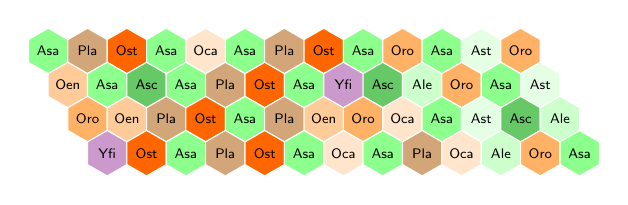
\begin{tikzpicture}[x=0.5cm,y=0.5cm,font=\sffamily\fontsize{4.5}{5}\selectfont]
  \filldraw[fill=green!45,draw=white,line width=0.4pt] (0.000,0.577) -- (-0.500,0.289) -- (-0.500,-0.289) -- (-0.000,-0.577) -- (0.500,-0.289) -- (0.500,0.289) -- cycle;
  \node at (0.000,0.000) {Asa};
  \filldraw[fill=brown!70,draw=white,line width=0.4pt] (1.000,0.577) -- (0.500,0.289) -- (0.500,-0.289) -- (1.000,-0.577) -- (1.500,-0.289) -- (1.500,0.289) -- cycle;
  \node at (1.000,0.000) {Pla};
  \filldraw[fill=orange!80!red,draw=white,line width=0.4pt] (2.000,0.577) -- (1.500,0.289) -- (1.500,-0.289) -- (2.000,-0.577) -- (2.500,-0.289) -- (2.500,0.289) -- cycle;
  \node at (2.000,0.000) {Ost};
  \filldraw[fill=green!45,draw=white,line width=0.4pt] (3.000,0.577) -- (2.500,0.289) -- (2.500,-0.289) -- (3.000,-0.577) -- (3.500,-0.289) -- (3.500,0.289) -- cycle;
  \node at (3.000,0.000) {Asa};
  \filldraw[fill=orange!20,draw=white,line width=0.4pt] (4.000,0.577) -- (3.500,0.289) -- (3.500,-0.289) -- (4.000,-0.577) -- (4.500,-0.289) -- (4.500,0.289) -- cycle;
  \node at (4.000,0.000) {Oca};
  \filldraw[fill=green!45,draw=white,line width=0.4pt] (5.000,0.577) -- (4.500,0.289) -- (4.500,-0.289) -- (5.000,-0.577) -- (5.500,-0.289) -- (5.500,0.289) -- cycle;
  \node at (5.000,0.000) {Asa};
  \filldraw[fill=brown!70,draw=white,line width=0.4pt] (6.000,0.577) -- (5.500,0.289) -- (5.500,-0.289) -- (6.000,-0.577) -- (6.500,-0.289) -- (6.500,0.289) -- cycle;
  \node at (6.000,0.000) {Pla};
  \filldraw[fill=orange!80!red,draw=white,line width=0.4pt] (7.000,0.577) -- (6.500,0.289) -- (6.500,-0.289) -- (7.000,-0.577) -- (7.500,-0.289) -- (7.500,0.289) -- cycle;
  \node at (7.000,0.000) {Ost};
  \filldraw[fill=green!45,draw=white,line width=0.4pt] (8.000,0.577) -- (7.500,0.289) -- (7.500,-0.289) -- (8.000,-0.577) -- (8.500,-0.289) -- (8.500,0.289) -- cycle;
  \node at (8.000,0.000) {Asa};
  \filldraw[fill=orange!60,draw=white,line width=0.4pt] (9.000,0.577) -- (8.500,0.289) -- (8.500,-0.289) -- (9.000,-0.577) -- (9.500,-0.289) -- (9.500,0.289) -- cycle;
  \node at (9.000,0.000) {Oro};
  \filldraw[fill=green!45,draw=white,line width=0.4pt] (10.000,0.577) -- (9.500,0.289) -- (9.500,-0.289) -- (10.000,-0.577) -- (10.500,-0.289) -- (10.500,0.289) -- cycle;
  \node at (10.000,0.000) {Asa};
  \filldraw[fill=green!10,draw=white,line width=0.4pt] (11.000,0.577) -- (10.500,0.289) -- (10.500,-0.289) -- (11.000,-0.577) -- (11.500,-0.289) -- (11.500,0.289) -- cycle;
  \node at (11.000,0.000) {Ast};
  \filldraw[fill=orange!60,draw=white,line width=0.4pt] (12.000,0.577) -- (11.500,0.289) -- (11.500,-0.289) -- (12.000,-0.577) -- (12.500,-0.289) -- (12.500,0.289) -- cycle;
  \node at (12.000,0.000) {Oro};
  \filldraw[fill=orange!40,draw=white,line width=0.4pt] (0.500,-0.289) -- (-0.000,-0.577) -- (0.000,-1.155) -- (0.500,-1.443) -- (1.000,-1.155) -- (1.000,-0.577) -- cycle;
  \node at (0.500,-0.866) {Oen};
  \filldraw[fill=green!45,draw=white,line width=0.4pt] (1.500,-0.289) -- (1.000,-0.577) -- (1.000,-1.155) -- (1.500,-1.443) -- (2.000,-1.155) -- (2.000,-0.577) -- cycle;
  \node at (1.500,-0.866) {Asa};
  \filldraw[fill=green!65!black!60,draw=white,line width=0.4pt] (2.500,-0.289) -- (2.000,-0.577) -- (2.000,-1.155) -- (2.500,-1.443) -- (3.000,-1.155) -- (3.000,-0.577) -- cycle;
  \node at (2.500,-0.866) {Asc};
  \filldraw[fill=green!45,draw=white,line width=0.4pt] (3.500,-0.289) -- (3.000,-0.577) -- (3.000,-1.155) -- (3.500,-1.443) -- (4.000,-1.155) -- (4.000,-0.577) -- cycle;
  \node at (3.500,-0.866) {Asa};
  \filldraw[fill=brown!70,draw=white,line width=0.4pt] (4.500,-0.289) -- (4.000,-0.577) -- (4.000,-1.155) -- (4.500,-1.443) -- (5.000,-1.155) -- (5.000,-0.577) -- cycle;
  \node at (4.500,-0.866) {Pla};
  \filldraw[fill=orange!80!red,draw=white,line width=0.4pt] (5.500,-0.289) -- (5.000,-0.577) -- (5.000,-1.155) -- (5.500,-1.443) -- (6.000,-1.155) -- (6.000,-0.577) -- cycle;
  \node at (5.500,-0.866) {Ost};
  \filldraw[fill=green!45,draw=white,line width=0.4pt] (6.500,-0.289) -- (6.000,-0.577) -- (6.000,-1.155) -- (6.500,-1.443) -- (7.000,-1.155) -- (7.000,-0.577) -- cycle;
  \node at (6.500,-0.866) {Asa};
  \filldraw[fill=violet!40,draw=white,line width=0.4pt] (7.500,-0.289) -- (7.000,-0.577) -- (7.000,-1.155) -- (7.500,-1.443) -- (8.000,-1.155) -- (8.000,-0.577) -- cycle;
  \node at (7.500,-0.866) {Yfi};
  \filldraw[fill=green!65!black!60,draw=white,line width=0.4pt] (8.500,-0.289) -- (8.000,-0.577) -- (8.000,-1.155) -- (8.500,-1.443) -- (9.000,-1.155) -- (9.000,-0.577) -- cycle;
  \node at (8.500,-0.866) {Asc};
  \filldraw[fill=green!20,draw=white,line width=0.4pt] (9.500,-0.289) -- (9.000,-0.577) -- (9.000,-1.155) -- (9.500,-1.443) -- (10.000,-1.155) -- (10.000,-0.577) -- cycle;
  \node at (9.500,-0.866) {Ale};
  \filldraw[fill=orange!60,draw=white,line width=0.4pt] (10.500,-0.289) -- (10.000,-0.577) -- (10.000,-1.155) -- (10.500,-1.443) -- (11.000,-1.155) -- (11.000,-0.577) -- cycle;
  \node at (10.500,-0.866) {Oro};
  \filldraw[fill=green!45,draw=white,line width=0.4pt] (11.500,-0.289) -- (11.000,-0.577) -- (11.000,-1.155) -- (11.500,-1.443) -- (12.000,-1.155) -- (12.000,-0.577) -- cycle;
  \node at (11.500,-0.866) {Asa};
  \filldraw[fill=green!10,draw=white,line width=0.4pt] (12.500,-0.289) -- (12.000,-0.577) -- (12.000,-1.155) -- (12.500,-1.443) -- (13.000,-1.155) -- (13.000,-0.577) -- cycle;
  \node at (12.500,-0.866) {Ast};
  \filldraw[fill=orange!60,draw=white,line width=0.4pt] (1.000,-1.155) -- (0.500,-1.443) -- (0.500,-2.021) -- (1.000,-2.309) -- (1.500,-2.021) -- (1.500,-1.443) -- cycle;
  \node at (1.000,-1.732) {Oro};
  \filldraw[fill=orange!40,draw=white,line width=0.4pt] (2.000,-1.155) -- (1.500,-1.443) -- (1.500,-2.021) -- (2.000,-2.309) -- (2.500,-2.021) -- (2.500,-1.443) -- cycle;
  \node at (2.000,-1.732) {Oen};
  \filldraw[fill=brown!70,draw=white,line width=0.4pt] (3.000,-1.155) -- (2.500,-1.443) -- (2.500,-2.021) -- (3.000,-2.309) -- (3.500,-2.021) -- (3.500,-1.443) -- cycle;
  \node at (3.000,-1.732) {Pla};
  \filldraw[fill=orange!80!red,draw=white,line width=0.4pt] (4.000,-1.155) -- (3.500,-1.443) -- (3.500,-2.021) -- (4.000,-2.309) -- (4.500,-2.021) -- (4.500,-1.443) -- cycle;
  \node at (4.000,-1.732) {Ost};
  \filldraw[fill=green!45,draw=white,line width=0.4pt] (5.000,-1.155) -- (4.500,-1.443) -- (4.500,-2.021) -- (5.000,-2.309) -- (5.500,-2.021) -- (5.500,-1.443) -- cycle;
  \node at (5.000,-1.732) {Asa};
  \filldraw[fill=brown!70,draw=white,line width=0.4pt] (6.000,-1.155) -- (5.500,-1.443) -- (5.500,-2.021) -- (6.000,-2.309) -- (6.500,-2.021) -- (6.500,-1.443) -- cycle;
  \node at (6.000,-1.732) {Pla};
  \filldraw[fill=orange!40,draw=white,line width=0.4pt] (7.000,-1.155) -- (6.500,-1.443) -- (6.500,-2.021) -- (7.000,-2.309) -- (7.500,-2.021) -- (7.500,-1.443) -- cycle;
  \node at (7.000,-1.732) {Oen};
  \filldraw[fill=orange!60,draw=white,line width=0.4pt] (8.000,-1.155) -- (7.500,-1.443) -- (7.500,-2.021) -- (8.000,-2.309) -- (8.500,-2.021) -- (8.500,-1.443) -- cycle;
  \node at (8.000,-1.732) {Oro};
  \filldraw[fill=orange!20,draw=white,line width=0.4pt] (9.000,-1.155) -- (8.500,-1.443) -- (8.500,-2.021) -- (9.000,-2.309) -- (9.500,-2.021) -- (9.500,-1.443) -- cycle;
  \node at (9.000,-1.732) {Oca};
  \filldraw[fill=green!45,draw=white,line width=0.4pt] (10.000,-1.155) -- (9.500,-1.443) -- (9.500,-2.021) -- (10.000,-2.309) -- (10.500,-2.021) -- (10.500,-1.443) -- cycle;
  \node at (10.000,-1.732) {Asa};
  \filldraw[fill=green!10,draw=white,line width=0.4pt] (11.000,-1.155) -- (10.500,-1.443) -- (10.500,-2.021) -- (11.000,-2.309) -- (11.500,-2.021) -- (11.500,-1.443) -- cycle;
  \node at (11.000,-1.732) {Ast};
  \filldraw[fill=green!65!black!60,draw=white,line width=0.4pt] (12.000,-1.155) -- (11.500,-1.443) -- (11.500,-2.021) -- (12.000,-2.309) -- (12.500,-2.021) -- (12.500,-1.443) -- cycle;
  \node at (12.000,-1.732) {Asc};
  \filldraw[fill=green!20,draw=white,line width=0.4pt] (13.000,-1.155) -- (12.500,-1.443) -- (12.500,-2.021) -- (13.000,-2.309) -- (13.500,-2.021) -- (13.500,-1.443) -- cycle;
  \node at (13.000,-1.732) {Ale};
  \filldraw[fill=violet!40,draw=white,line width=0.4pt] (1.500,-2.021) -- (1.000,-2.309) -- (1.000,-2.887) -- (1.500,-3.175) -- (2.000,-2.887) -- (2.000,-2.309) -- cycle;
  \node at (1.500,-2.598) {Yfi};
  \filldraw[fill=orange!80!red,draw=white,line width=0.4pt] (2.500,-2.021) -- (2.000,-2.309) -- (2.000,-2.887) -- (2.500,-3.175) -- (3.000,-2.887) -- (3.000,-2.309) -- cycle;
  \node at (2.500,-2.598) {Ost};
  \filldraw[fill=green!45,draw=white,line width=0.4pt] (3.500,-2.021) -- (3.000,-2.309) -- (3.000,-2.887) -- (3.500,-3.175) -- (4.000,-2.887) -- (4.000,-2.309) -- cycle;
  \node at (3.500,-2.598) {Asa};
  \filldraw[fill=brown!70,draw=white,line width=0.4pt] (4.500,-2.021) -- (4.000,-2.309) -- (4.000,-2.887) -- (4.500,-3.175) -- (5.000,-2.887) -- (5.000,-2.309) -- cycle;
  \node at (4.500,-2.598) {Pla};
  \filldraw[fill=orange!80!red,draw=white,line width=0.4pt] (5.500,-2.021) -- (5.000,-2.309) -- (5.000,-2.887) -- (5.500,-3.175) -- (6.000,-2.887) -- (6.000,-2.309) -- cycle;
  \node at (5.500,-2.598) {Ost};
  \filldraw[fill=green!45,draw=white,line width=0.4pt] (6.500,-2.021) -- (6.000,-2.309) -- (6.000,-2.887) -- (6.500,-3.175) -- (7.000,-2.887) -- (7.000,-2.309) -- cycle;
  \node at (6.500,-2.598) {Asa};
  \filldraw[fill=orange!20,draw=white,line width=0.4pt] (7.500,-2.021) -- (7.000,-2.309) -- (7.000,-2.887) -- (7.500,-3.175) -- (8.000,-2.887) -- (8.000,-2.309) -- cycle;
  \node at (7.500,-2.598) {Oca};
  \filldraw[fill=green!45,draw=white,line width=0.4pt] (8.500,-2.021) -- (8.000,-2.309) -- (8.000,-2.887) -- (8.500,-3.175) -- (9.000,-2.887) -- (9.000,-2.309) -- cycle;
  \node at (8.500,-2.598) {Asa};
  \filldraw[fill=brown!70,draw=white,line width=0.4pt] (9.500,-2.021) -- (9.000,-2.309) -- (9.000,-2.887) -- (9.500,-3.175) -- (10.000,-2.887) -- (10.000,-2.309) -- cycle;
  \node at (9.500,-2.598) {Pla};
  \filldraw[fill=orange!20,draw=white,line width=0.4pt] (10.500,-2.021) -- (10.000,-2.309) -- (10.000,-2.887) -- (10.500,-3.175) -- (11.000,-2.887) -- (11.000,-2.309) -- cycle;
  \node at (10.500,-2.598) {Oca};
  \filldraw[fill=green!20,draw=white,line width=0.4pt] (11.500,-2.021) -- (11.000,-2.309) -- (11.000,-2.887) -- (11.500,-3.175) -- (12.000,-2.887) -- (12.000,-2.309) -- cycle;
  \node at (11.500,-2.598) {Ale};
  \filldraw[fill=orange!60,draw=white,line width=0.4pt] (12.500,-2.021) -- (12.000,-2.309) -- (12.000,-2.887) -- (12.500,-3.175) -- (13.000,-2.887) -- (13.000,-2.309) -- cycle;
  \node at (12.500,-2.598) {Oro};
  \filldraw[fill=green!45,draw=white,line width=0.4pt] (13.500,-2.021) -- (13.000,-2.309) -- (13.000,-2.887) -- (13.500,-3.175) -- (14.000,-2.887) -- (14.000,-2.309) -- cycle;
  \node at (13.500,-2.598) {Asa};
\end{tikzpicture}

\caption{Clave de plantación 1, compartida por 18 polígonos: mosaico de $4\times13$ posiciones al tresbolillo que se repite sobre el polígono; competencia 78.18 frente a 93.34 al azar. Verdes: \textit{Agave}; naranjas: \textit{Opuntia}; café: \textit{P.~laevigata}; morado: \textit{Y.~filifera}. Abreviaturas como en la \cref{tab:matriz-competencia}.}
\label{fig:clave1}
\end{figure}

\subsubsection{Sensibilidad a la matriz de competencia}
\label{subsec:res-sensibilidad}

La matriz $W$ depende de rasgos aproximados y de dos parámetros fijados por supuesto. Para medir cuánto dependen las claves de esos valores, se despejó el producto $T_{ab}N_{ab}$ de cada par a partir de la matriz base y de \eqref{eq:matriz-W}, con $\gamma=1.5$, $\phi=0.3$ y el efecto nodriza aplicado a los pares de \textit{P.~laevigata} con agaves y nopales\footnote{Con esa convención la reconstrucción devuelve exactamente la matriz base. Aplicarlo también a \textit{Y.~filifera} implicaría un traslape de raíces con el mezquite de 0.75, mayor que el de cualquier suculenta, lo que no corresponde a una roseta de raíz somera.}. Con ello se construyeron 45 matrices alternativas: 25 en la rejilla $\gamma\in\{1,1.25,1.5,1.75,2\}$, $\phi\in\{0,0.15,0.3,0.45,0.6\}$, y 20 en las que el producto $T_{ab}N_{ab}$ de cada par se multiplica por un factor uniforme e independiente en $[0.7,1.3]$, una perturbación más severa que variar el diámetro de copa de cada especie, porque afecta a cada par por separado. Con cada matriz se reoptimizaron los seis mosaicos (10 corridas del memético) y se comparó la competencia de la clave base, evaluada con la matriz alternativa, con la de la clave reoptimizada.

Las claves son robustas a $\gamma$ y $\phi$: en las 150 combinaciones de matriz y mosaico de la rejilla, la clave base queda a lo más 1.6\,\% por encima de la reoptimizada (mediana 0.15\,\%), y con $\gamma\geq1.25$ y $\phi\geq0.3$ es igual de buena. Solo con $\gamma=1$, es decir, sin penalización intraespecífica adicional, la diferencia supera el 1\,\%. Los rasgos pesan más. Con las matrices perturbadas, cuya correlación de Spearman con la base va de 0.91 a 0.95, la clave base queda en promedio 6.6\,\% por encima de la reoptimizada (máximo 11.6\,\%), aunque sigue reduciendo la competencia entre 9\,\% y 20\,\% respecto al azar. En la práctica, $\gamma$ y $\phi$ no necesitan precisarse más, pero vale la pena afinar los diámetros de copa y los perfiles de raíz antes de imprimir las claves.

\subsection{Discusión}
\label{subsec:discusion}

\paragraph{Lo que significa para CONAFOR} Con el presupuesto actual no es posible cumplir la meta en ningún polígono con una confiabilidad razonable; se necesitan alrededor de \$14{,}500/ha, o bien reducir la meta o la superficie. El modelo traduce esa decisión a números: \cref{tab:frontera} indica cuánto cuesta cada nivel de riesgo, y la diferencia entre niveles es pequeña frente al faltante. Lo que sí está en manos del planeador es la composición: agotar el margen de $\pm$10\,\% hacia los nopales es lo que hace la compra más barata. Si ese margen se redujera por razones ecológicas, el presupuesto necesario subiría.

\paragraph{Limitaciones} Los resultados dependen de supuestos que conviene revisar con el socio formador. La supervivencia se estimó con un solo año de monitoreo y se supone independiente entre plantas; un año seco afectaría a todas a la vez. Las plantas existentes se toman como un conteo exacto que no muere. La matriz de competencia se construyó con rasgos aproximados; las claves son robustas a $\gamma$ y $\phi$, pero no a errores grandes en los rasgos (\cref{subsec:res-sensibilidad}), y la matriz no se ha contrastado con observaciones de campo. Por último, el agua, la disponibilidad en vivero y el terreno de cada polígono quedaron fuera del modelo.

